% Source: graduate-coursework/Sp26/CSCE775/Project/proposal_radar_1/proposal1_radar.tex
% Description: Proposed system architecture. The SAC policy outputs both a structured scene program (object groups, paths, intensity profiles, flicker schedules, clutter settings) and trail rendering parameters ($N$, decay $f(k)$, encoding, color mapping). The EchoTrails generator produces raw PPI frames, which the trail renderer augments with temporal compositing. A YOLOv8n detector is trained on the augmented images and its validation mAP$_{50\text{-

\documentclass[border=4pt]{standalone}
\usepackage{amsmath,amssymb}
\usepackage{graphicx}
\usepackage{tikz}
\usetikzlibrary{positioning, arrows.meta, shapes.geometric, fit, calc, backgrounds}

\begin{document}
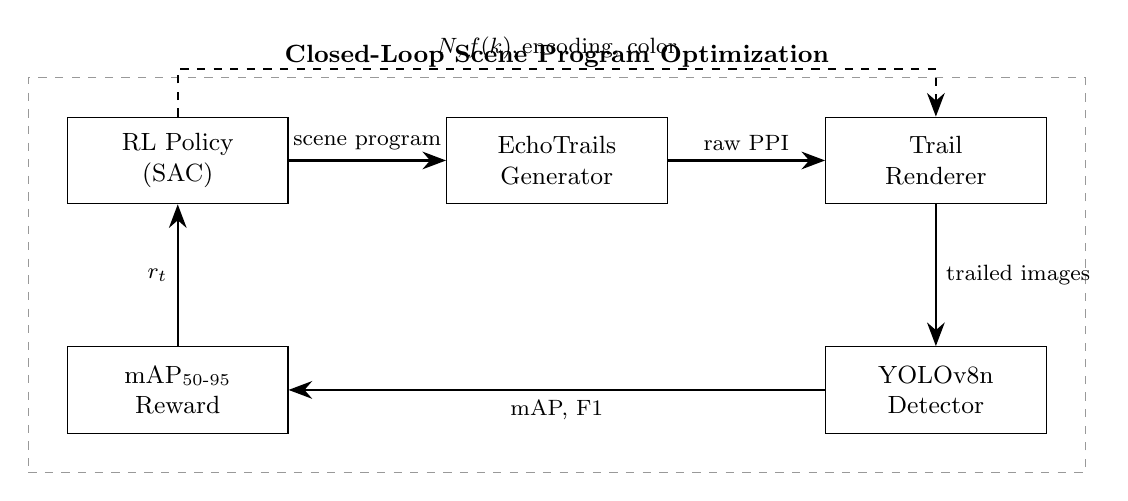
\begin{tikzpicture}[
    block/.style={draw, minimum width=2.8cm, minimum height=1.1cm, align=center, font=\small},
    data/.style={draw, minimum width=2.2cm, minimum height=0.9cm, align=center, font=\small, dashed},
    arr/.style={-{Stealth[length=3mm]}, thick},
    every node/.style={font=\small}
]

% RL Agent
\node[block, fill=white] (agent) {RL Policy\\(SAC)};

% Generator
\node[block, fill=white, right=2.0cm of agent] (gen) {EchoTrails\\Generator};

% Trail Renderer
\node[block, fill=white, right=2.0cm of gen] (trail) {Trail\\Renderer};

% Downstream Model
\node[block, fill=white, below=1.8cm of trail] (model) {YOLOv8n\\Detector};

% Validation Score
\node[block, fill=white, below=1.8cm of agent] (val) {mAP$_{50\text{-}95}$\\Reward};

% Arrows
\draw[arr] (agent) -- node[above, font=\footnotesize] {scene program} (gen);
\draw[arr] (gen) -- node[above, font=\footnotesize] {raw PPI} (trail);
\draw[arr] (trail) -- node[right, font=\footnotesize] {trailed images} (model);
\draw[arr] (model) -- node[below, font=\footnotesize] {mAP, F1} (val);
\draw[arr] (val) -- node[left, font=\footnotesize] {$r_t$} (agent);

% Curved arrow for trail params
\draw[arr, dashed] (agent.north) -- ++(0,0.6) -| node[above, pos=0.25, font=\footnotesize] {$N, f(k), \text{encoding, color}$} (trail.north);

% Background box
\begin{scope}[on background layer]
\node[draw=black!40, dashed, inner sep=14pt, fit=(agent)(gen)(trail)(model)(val), label={[font=\small\bfseries]above:Closed-Loop Scene Program Optimization}] {};
\end{scope}

\end{tikzpicture}
\end{document}
